%%% SVN stuff
\svnidlong
{$HeadURL: https://svn.riouxsvn.com/kneadlatxinputs/ExampleArtifactFolders/6a%20-%20STP/STP_Chapter_01.tex $}
{$LastChangedDate: 2024-01-04 08:33:07 -0500 (Thu, 04 Jan 2024) $}
{$LastChangedRevision: 54 $}
{$LastChangedBy: KneadProject $}
\svnid{$Id: STP_Chapter_01.tex 54 2024-01-04 13:33:07Z KneadProject $}

\chapter{Scope}
\label{loc:Scope}
\DIDINFO{ALL-1.0 :: If applicable, each section has a summary of data item description (DID) information shown in this font.
These are displayed in small capital font and are not part of the formal document.
Display of these DID information notes can be turned off for formal releases, but are displayed here for reference.}



This document provides the System Test Plan (\STP) for the \ThisSystem, which is known as \ThisSys.
These engineering tests provide the multistage plan for testing of the \ThisSys, which follows Appendix A of DOD-STD-2106 (Navy)~\cite{ref__DOD_STD_2106_NAVY}.


\section{Identification}
\DIDINFO{ALL-1.1 :: This paragraph shall contain a full identification of the system to which this document applies, including, as applicable, identification number(s), title(s), abbreviation(s), version number(s), and release number(s).}

The \ThisSys, described in this document shall be known as \ThisSys version 1.0.


\section{System Overview}
\label{loc:SystemOverview}
\DIDINFO{ALL-1.2 :: This paragraph shall briefly state the purpose of the system to which this document applies. It shall describe the general nature of the system; summarize the history of system development, operation, and maintenance; identify the project sponsor, acquirer, user, developer, and support agencies; identify current and planned operating sites; and list other relevant documents.}

The \ThisSystem system is \TBD.

Figure~\ref{fig:SystemOverview} shows the high-level architecture for the \ThisSys system. 
\begin{figure}[htbp]
	\centering
		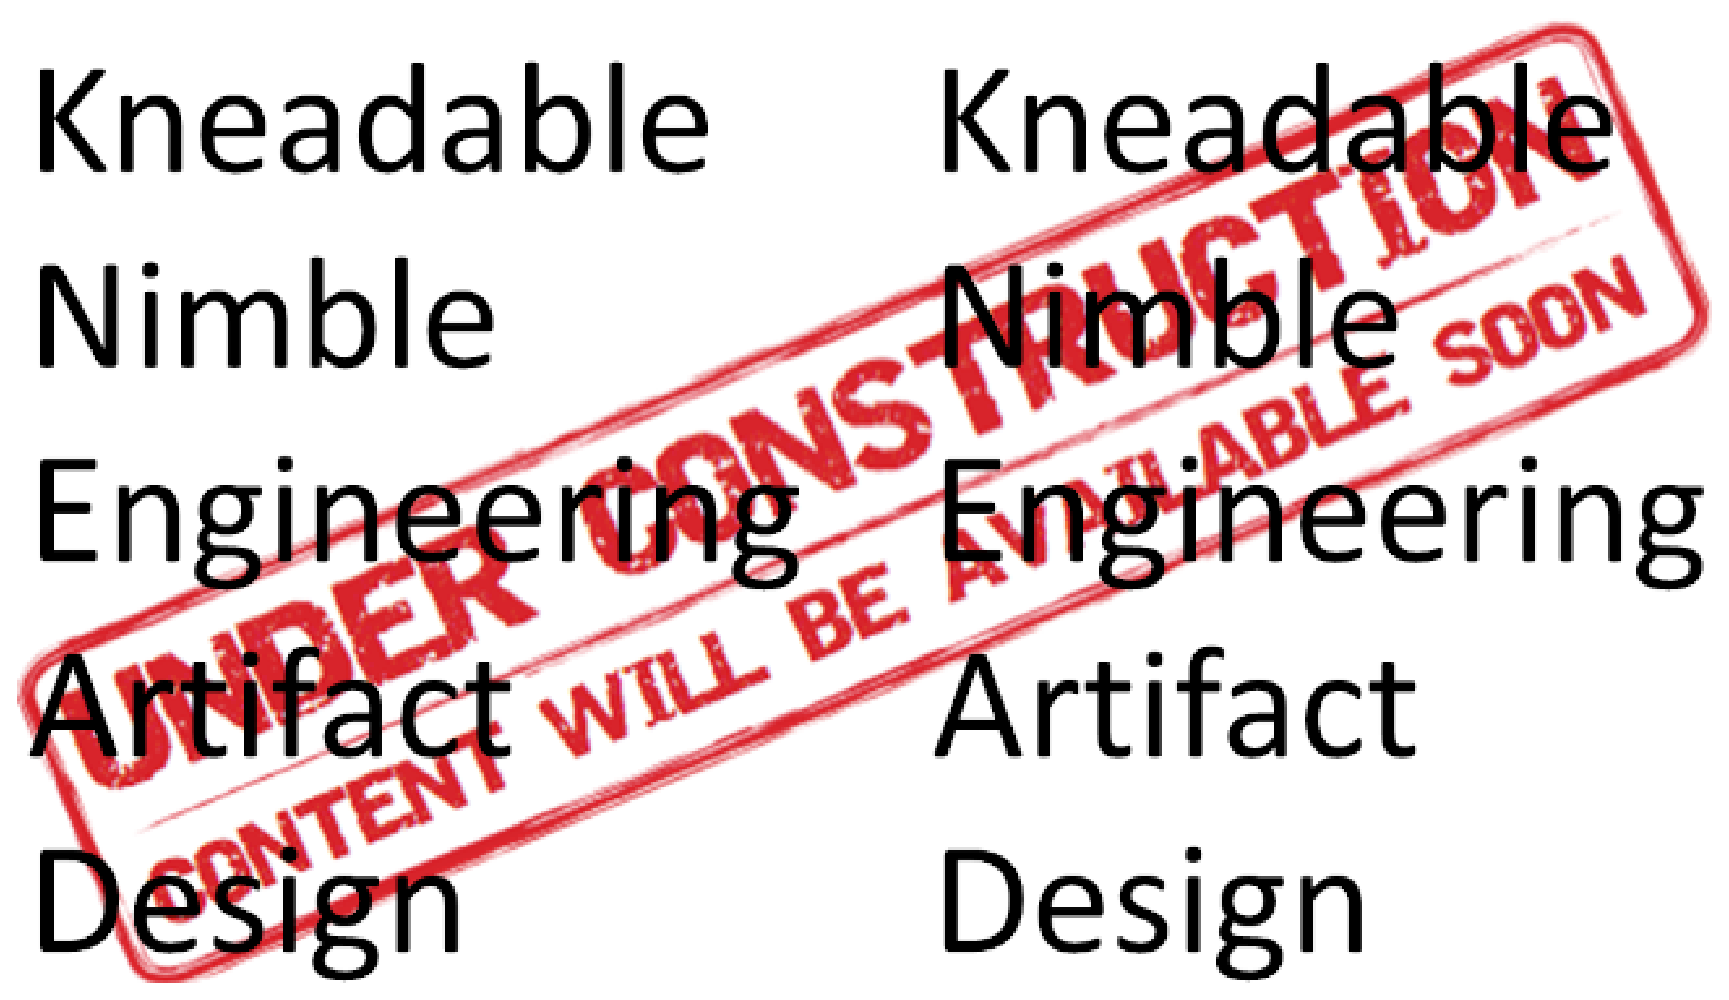
\includegraphics[width=6in]{images/KNEAD_UnderConstruction_100dpi_6.5inchesWide.eps}
		\caption{System Overview}
	\label{fig:SystemOverview}
\end{figure}
This diagram shows the major external interfaces that provide the capabilities of \ThisSys.
As are shown, the \ThisSys can provide. This system's main goal is to automate functionality
in order to make great Espresso.


The general concept of operations (\CONOP) for this system is User Selects an input weight through
an OLED screen using a rotery encoder. Espresso is prepared. User begins a shot, solid state relays 
are enabled and the shot begins to pull and a timer is started. As water falls into the cup and onto 
the load cells, the espresso cup is weighed. Once the desired weight is met the pump is turned off.
The user is displayed their time and weight on the OLED screen and data is pushed \TBD

While the system is not actively pulling a shot, it will be monitoring the water level. If low water
is detected the user will be notified.








\section{Document Overview}
\label{loc:DocumentOverview}
\DIDINFO{ALL-1.3 :: This paragraph shall summarize the purpose and contents of this
document and shall describe any security or privacy considerations associated with its use.}

This section provides information about this document's security/privacy considerations, contents, structure, and version information.

\subsection{Security and Privacy Considerations}
\label{loc:DocOverview_CUI}

This document has been identified as "Controlled Unclassified Information" (\CUI).
Please follow the control block on the title page for ownership, creation, category, dissemination, and Point of Contact (\POC) information.
This information should be delineated, per \url{https://www.dodcui.mil} as:
\begin{description}[itemindent=5pt,topsep=0pt,itemsep=0pt,partopsep=0pt, parsep=0pt]
	\item[Owner] the name of the DoD Component (not required if identified in the letterhead)
	\item[Creator] identification of the office creating the document
	\item[Category] identification of the categories contained in the document
	\item[Dissemination]applicable distribution statement or limited dissemination control (LDC)
	\item[\POC]name and phone number or email of POC
\end{description}


This document format is based upon the guidance in the \OCD{} \DID~\cite{ref__OCD_DID}.
The operational concept is documented following the guidelines of ISO-12207~\cite{ref__ISO_12207} and MIL-STD-498~\cite{ref__MIL_STD_498} (from which ISO-12207 originated).
This document follows the listed \OCD sub-section order.
\begin{description}[itemsep=-1ex,topsep=0pt]
	\item[Section 1] provides an overview of the system and this document.
	\item[Section 2] lists general and application-specific reference documents as well as glossary terms and acronyms. 
	\item[Section 3] summarizes the current status into which this system is to be situated.
	\item[Section 4] justifies why change is needed. 
	\item[Section 5] describes the concept for a new or modified system.
	\item[Section 6] illustrates operational scenarios for the new or modified system.
	\item[Section 7] discusses a summary of impacts for the new system.
	\item[Section 8] details analysis of the proposed system.
	\item[Appendices] if needed, provide additional information as may be needed.
\end{description}

\vspace{12pt}
\DIDINFO{If this text is visible, the first instance of each section may display a summary of data item description (DID) information shown in this font.
These are displayed in small capital font and are not part of the formal document.}


\subsection{Document Version Information}
\label{loc:DocOverview_LaTeXAndSvnVersionInformation}

This document was produced in \LaTeXx and \Biberx.
The editing and document preparation were performed using MiK\TeX{} version 2.9  with the build option $[$\LaTeX{}  $\Rightarrow$ PS $\Rightarrow$ PDF$]$.
The \LaTeXx {\em svn-multi} package was used to glean SVN tracking information, when files are stored in an ``SVN'' version control system.
The style {\tt \KNEADdocumentClsName}
%, which was based on the style provided in~\cite{ref__thesisguide}, 
was used to provide the \LaTeXx and \Biberx formatting details.

This revision of this document has the following properties:
\begin{table}[htbp]
	% \caption{Subversion (SVN) Data}
	% \label{tab:SVNdata}
	\centering
		\begin{tabular}{|p{1.5in}|p{4.9in}|}
		%%%%%S\multicolumn{2}{c}{\bfseries SVN Information} \\
		\hline
			{\bfseries Tracking Item}  &  {\bfseries Data} \\
		\hline		
		\hline
			Repository         & \url{\svnmainurl}  \\
		\hline
			Author         & \svnauthor  \\			
		\hline
			Revision       & \svnrev     \\	
		\hline
			Rev Date       & \svndate    \\	
		\hline	
			Print Date     & \today{} \currenttime    \\	
		\hline
			\KNEADdocumentClsName\break Version     & \KNEADdocumentClsVersion    \\	
		\hline	
			\KNEADdocumentClsName\break Date        & \KNEADdocumentClsDate   \\	
		\hline
		%%%\DocumentTexName\break Version     & \DocumentTexVersion    \\	
		%%%\hline	
		%%%\DocumentTexName\break Date        & \DocumentTexDate   \\	
		\hline						
    \end{tabular}
\end{table}


